\subsubsection{\large Diagrama de flujo \texttt{(conexion.c)}}
% --- PROCEDIMIENTO 1 ---
\newpage
\paragraph{1. Procedimiento \texttt{conexion()}} ~\\
\begin{figure}[H]
    \centering
    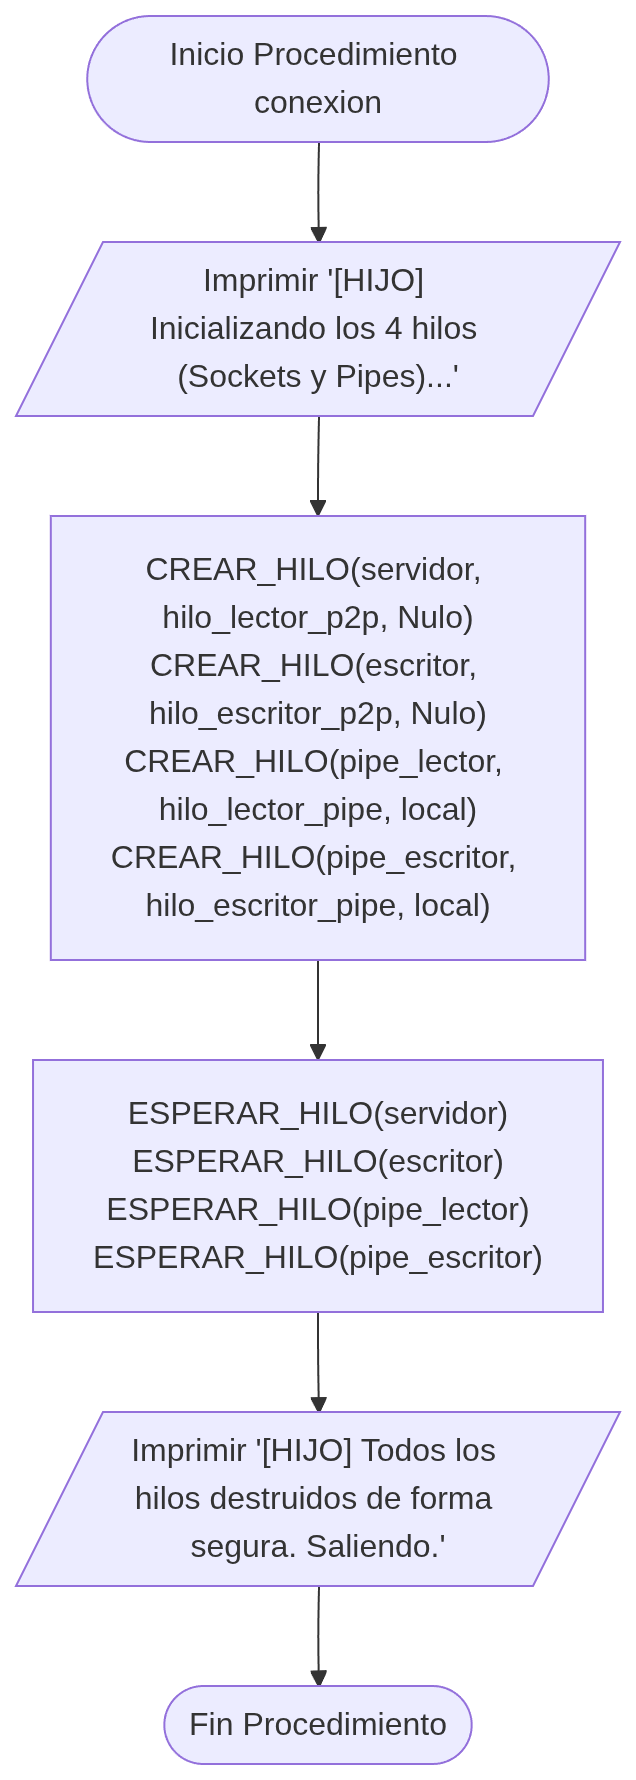
\includegraphics[width=0.25\textwidth]{Diagramas2/conexion.png} 
\end{figure}

% --- FUNCION 2 ---
\newpage
\paragraph{2.Función \texttt{hilo\_lector\_p2p()}} ~\\
\begin{figure}[H]
    \centering
    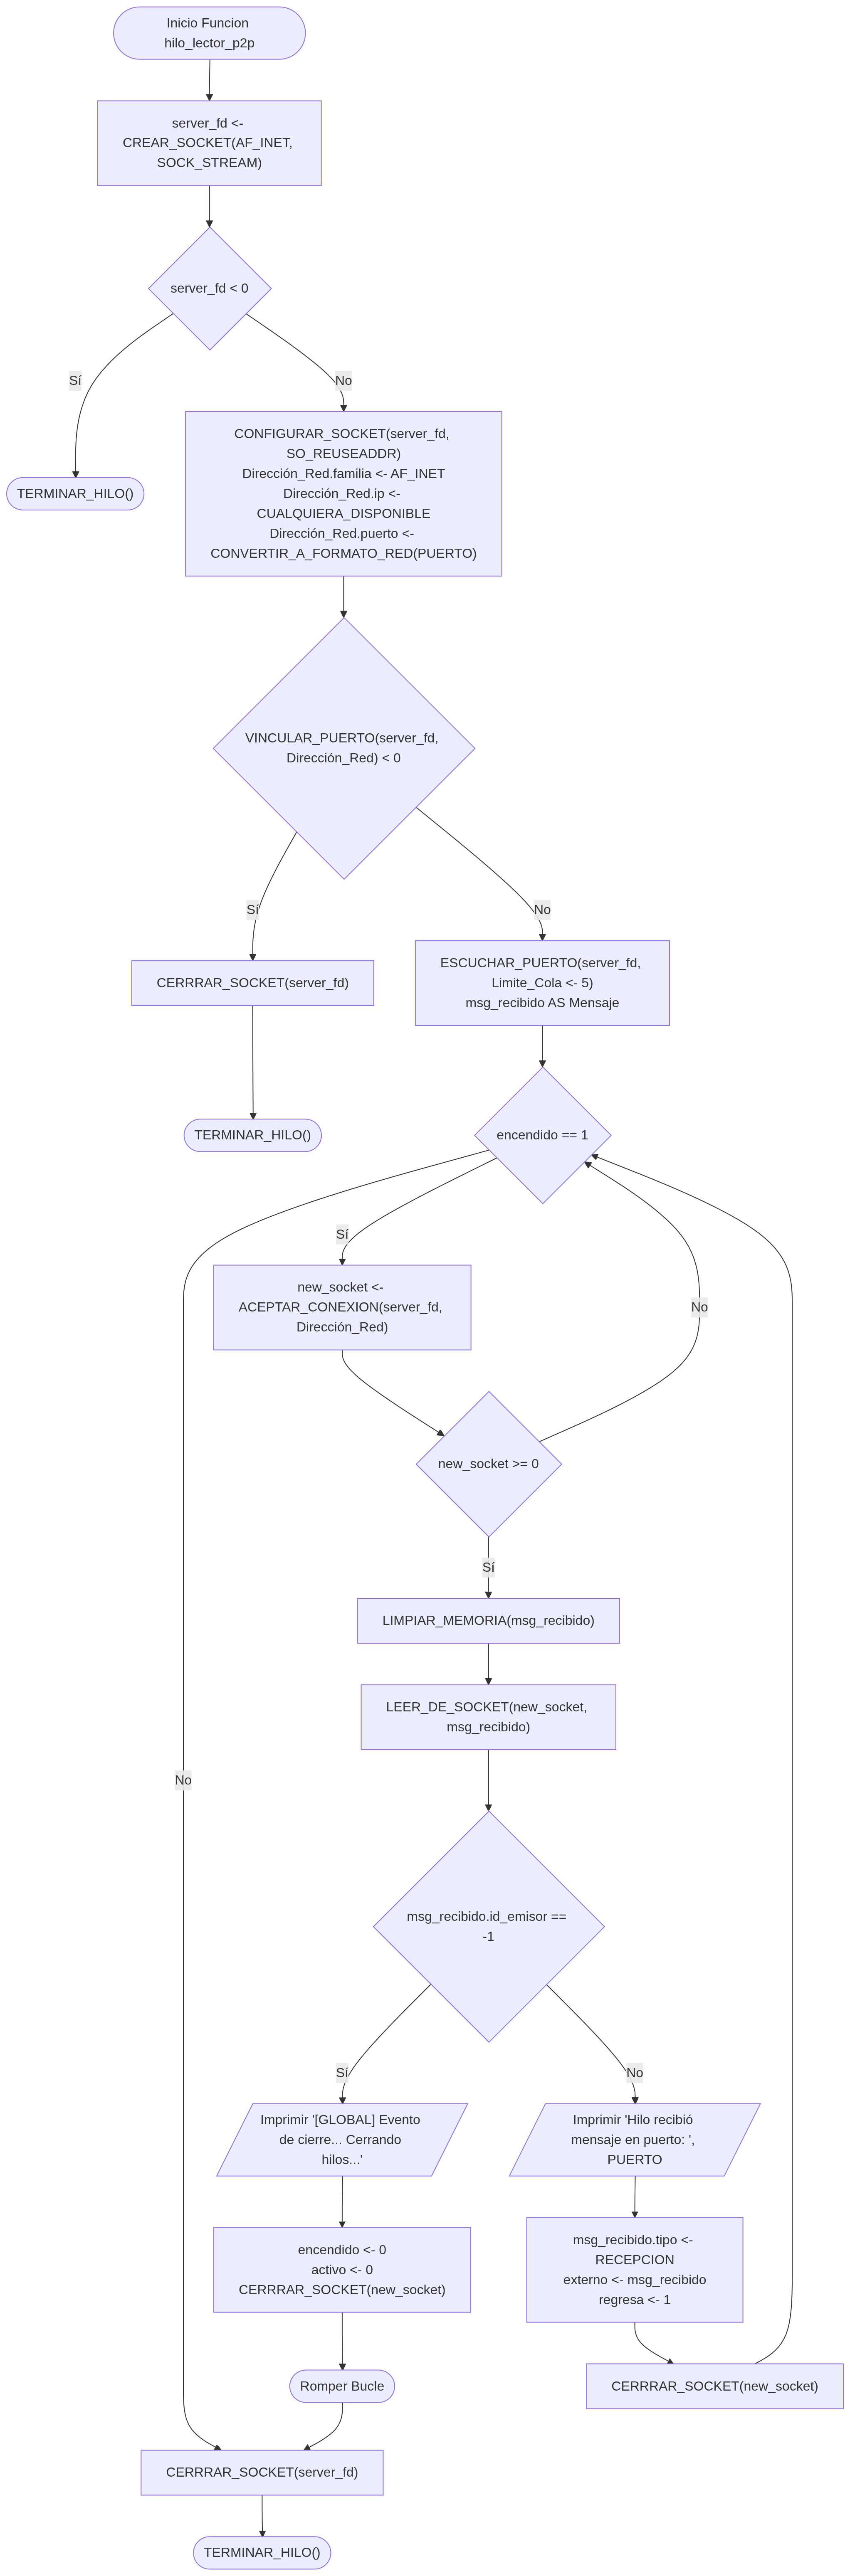
\includegraphics[width=0.35\textwidth]{Diagramas2/hilo_lector_p2p.png} 
\end{figure}

% --- FUNCION 3 ---
\newpage
\paragraph{3. Función \texttt{hilo\_escritor\_p2p()}} ~\\
\begin{figure}[H]
    \centering
    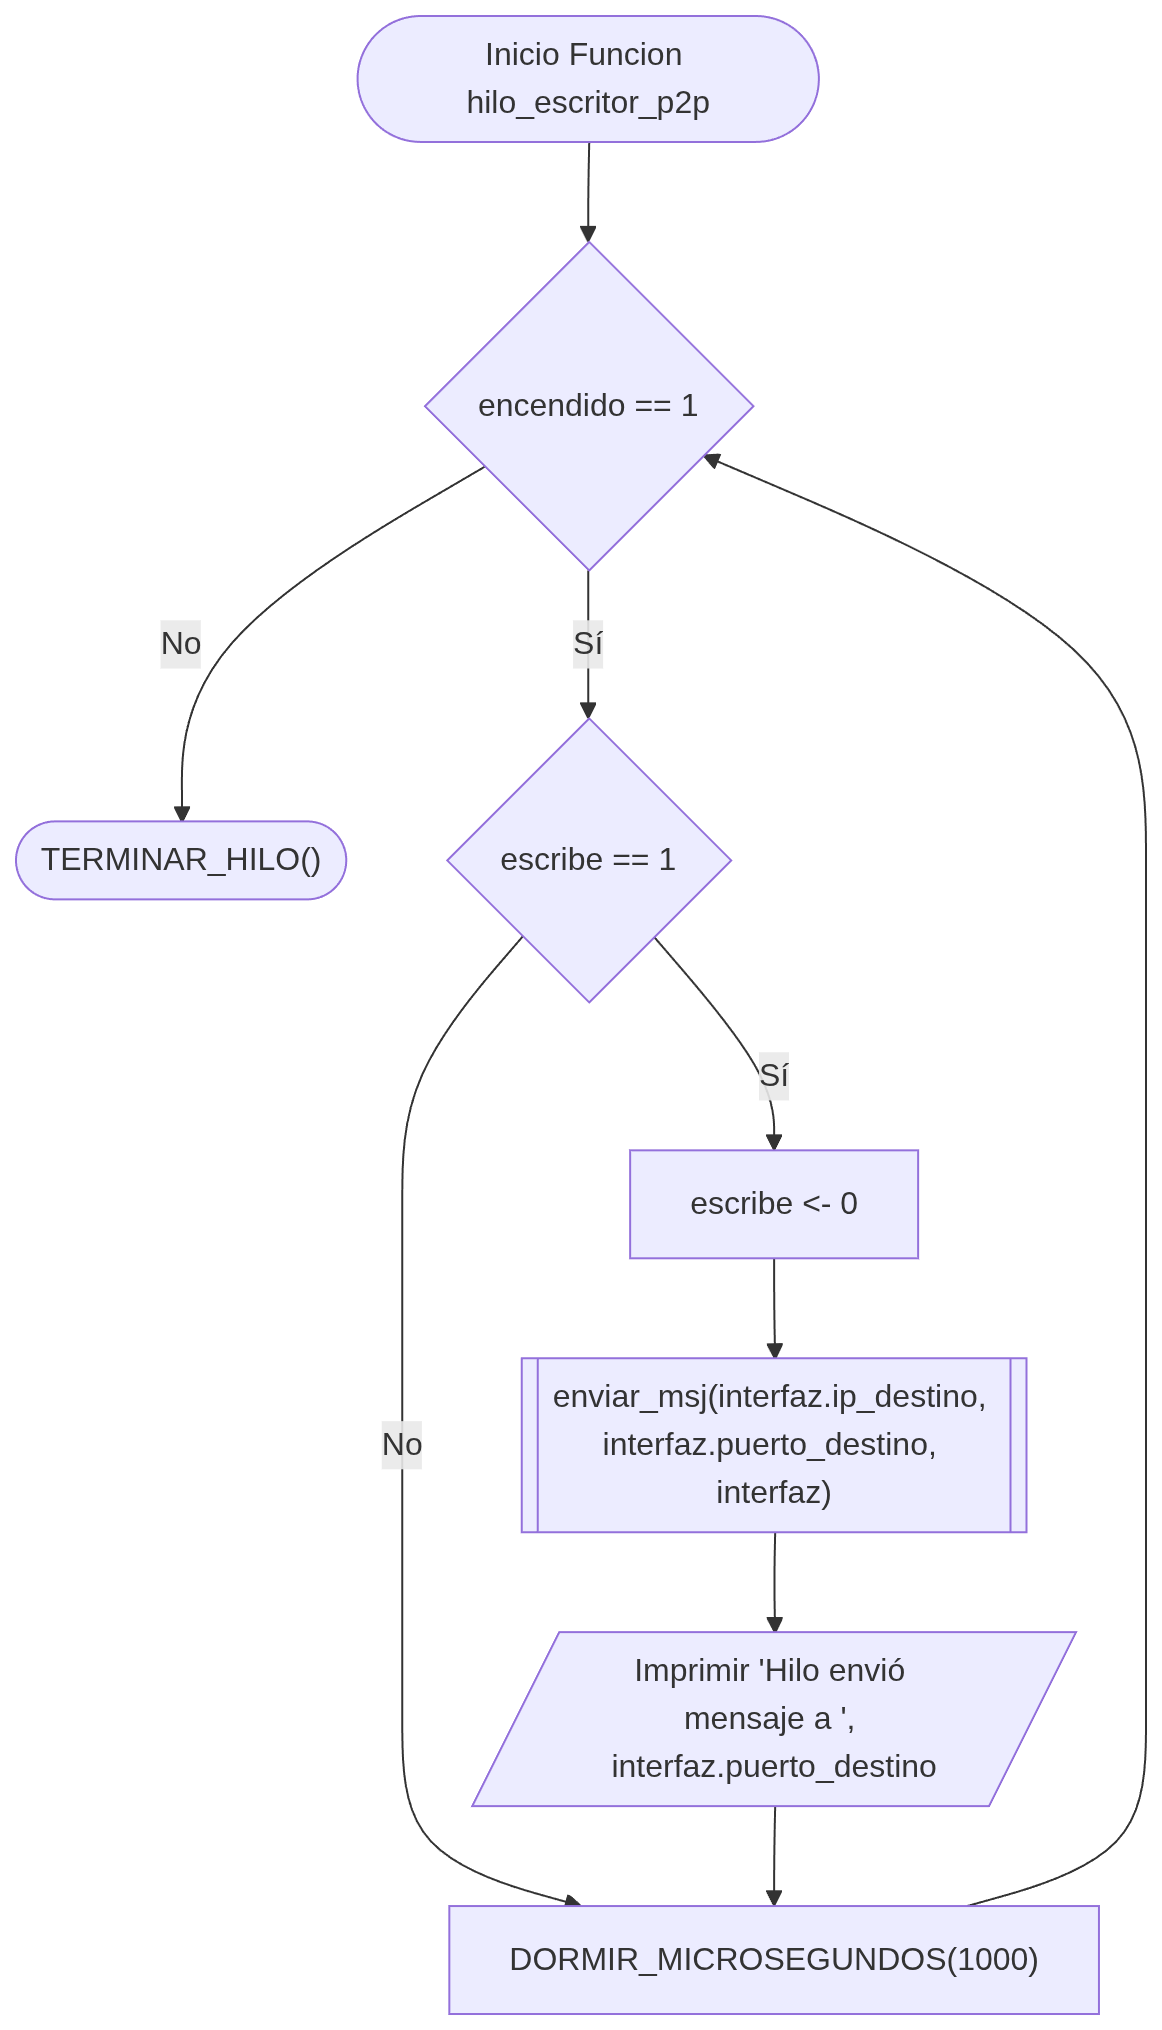
\includegraphics[width=0.4\textwidth]{Diagramas2/hilo_escritor_p2p.png} 
\end{figure}

% --- FUNCION 4 ---
\newpage
\paragraph{4. Función \texttt{hilo\_lector\_pipe()}} ~\\
\begin{figure}[H]
    \centering
    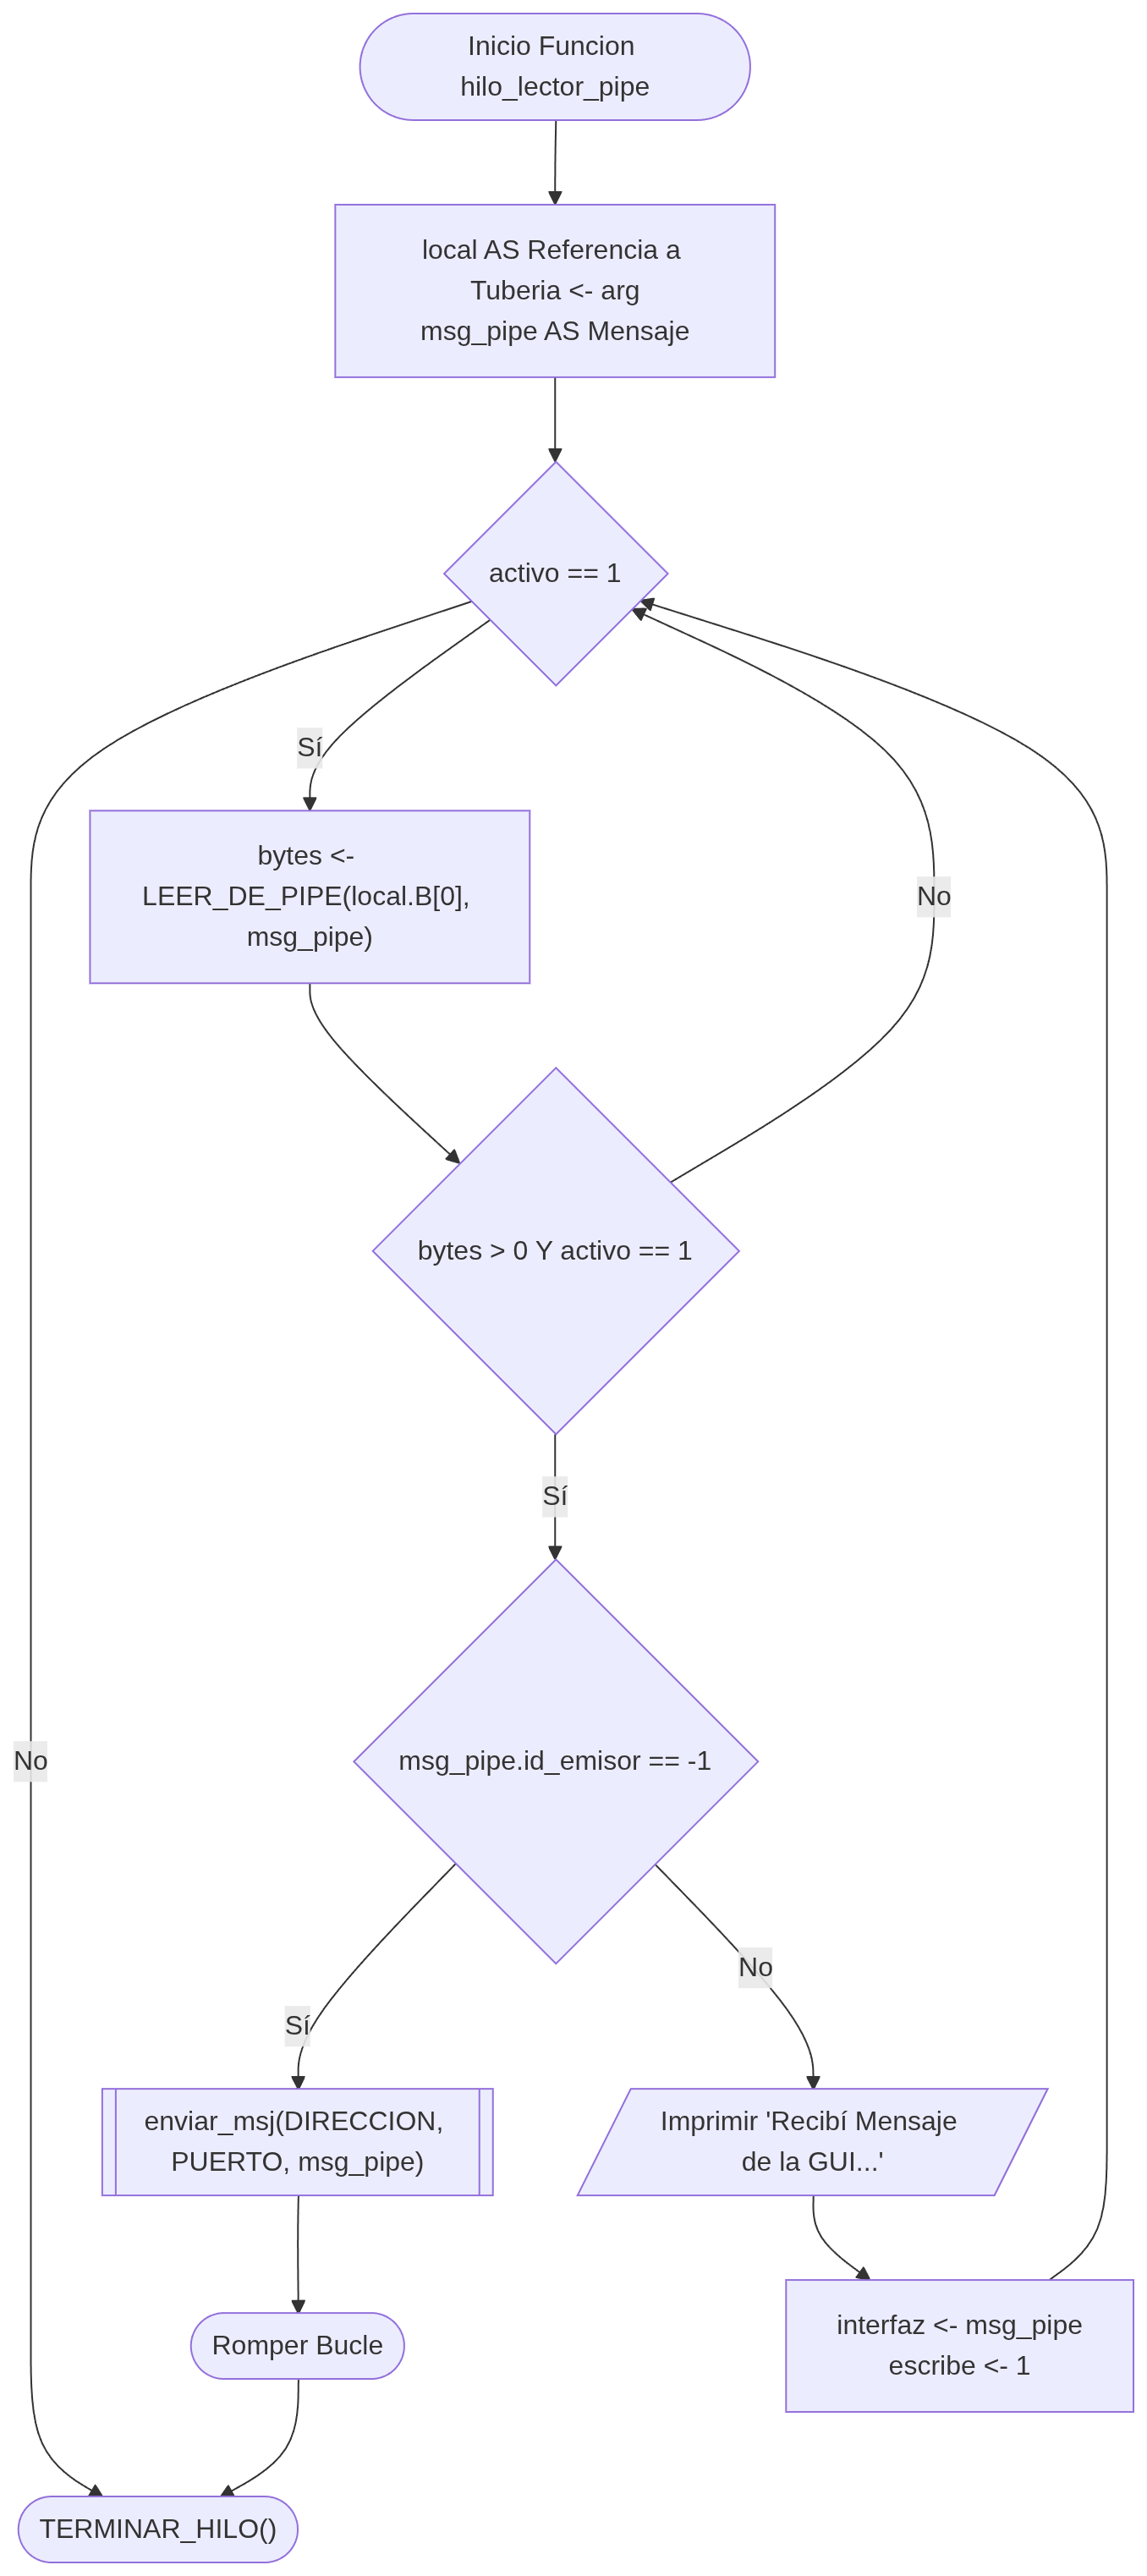
\includegraphics[width=0.4\textwidth]{Diagramas2/hilo_lector_pipe.png} 
\end{figure}

% --- FUNCION 5 ---
\newpage
\paragraph{5. Función \texttt{hilo\_escritor\_pipe()}} ~\\
\begin{figure}[H]
    \centering
    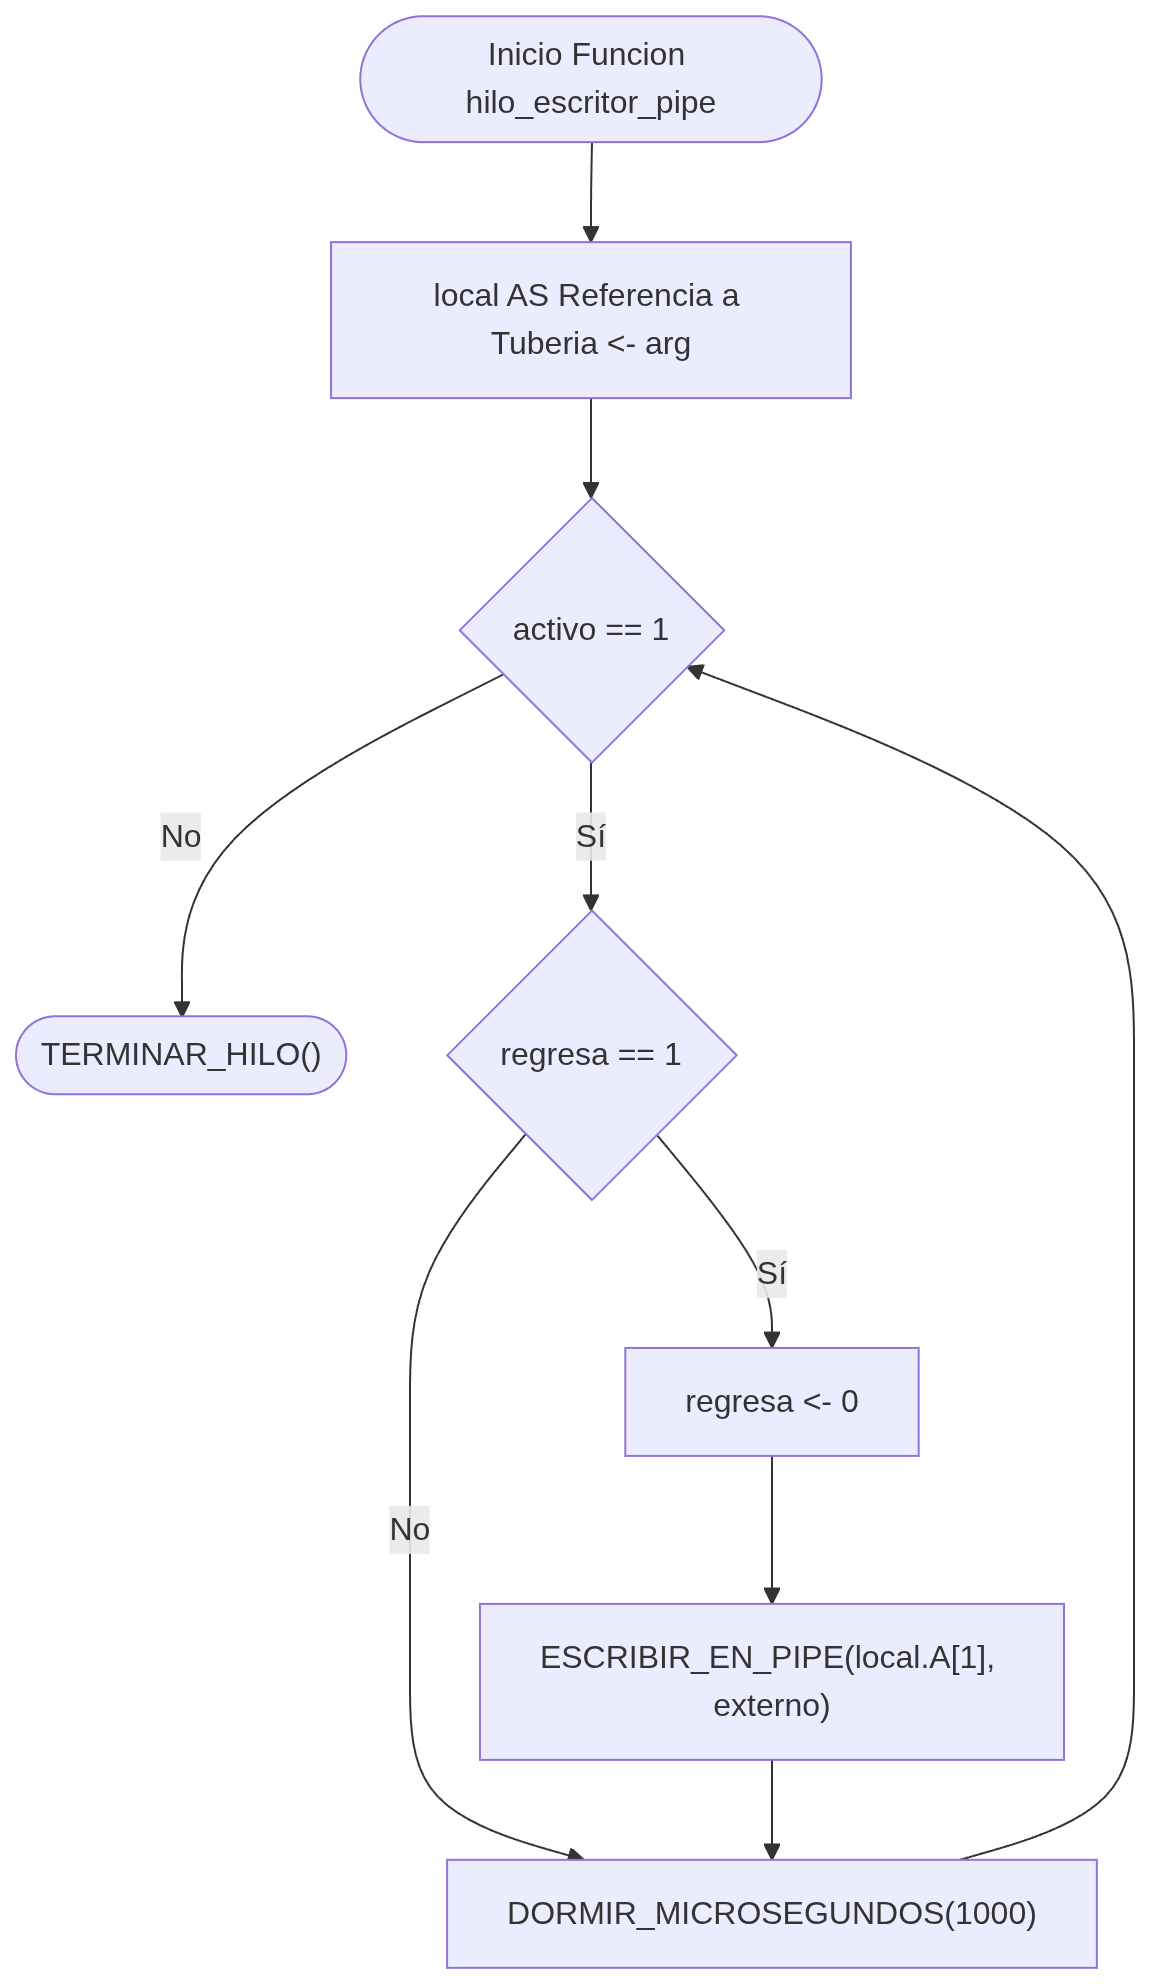
\includegraphics[width=0.4\textwidth]{Diagramas2/hilo_escritor_pipe.png} 
\end{figure}

% --- PROCEDIMIENTO 6 ---
\newpage
\paragraph{6. Procedimiento \texttt{enviar\_msj()}} ~\\
\begin{figure}[H]
    \centering
    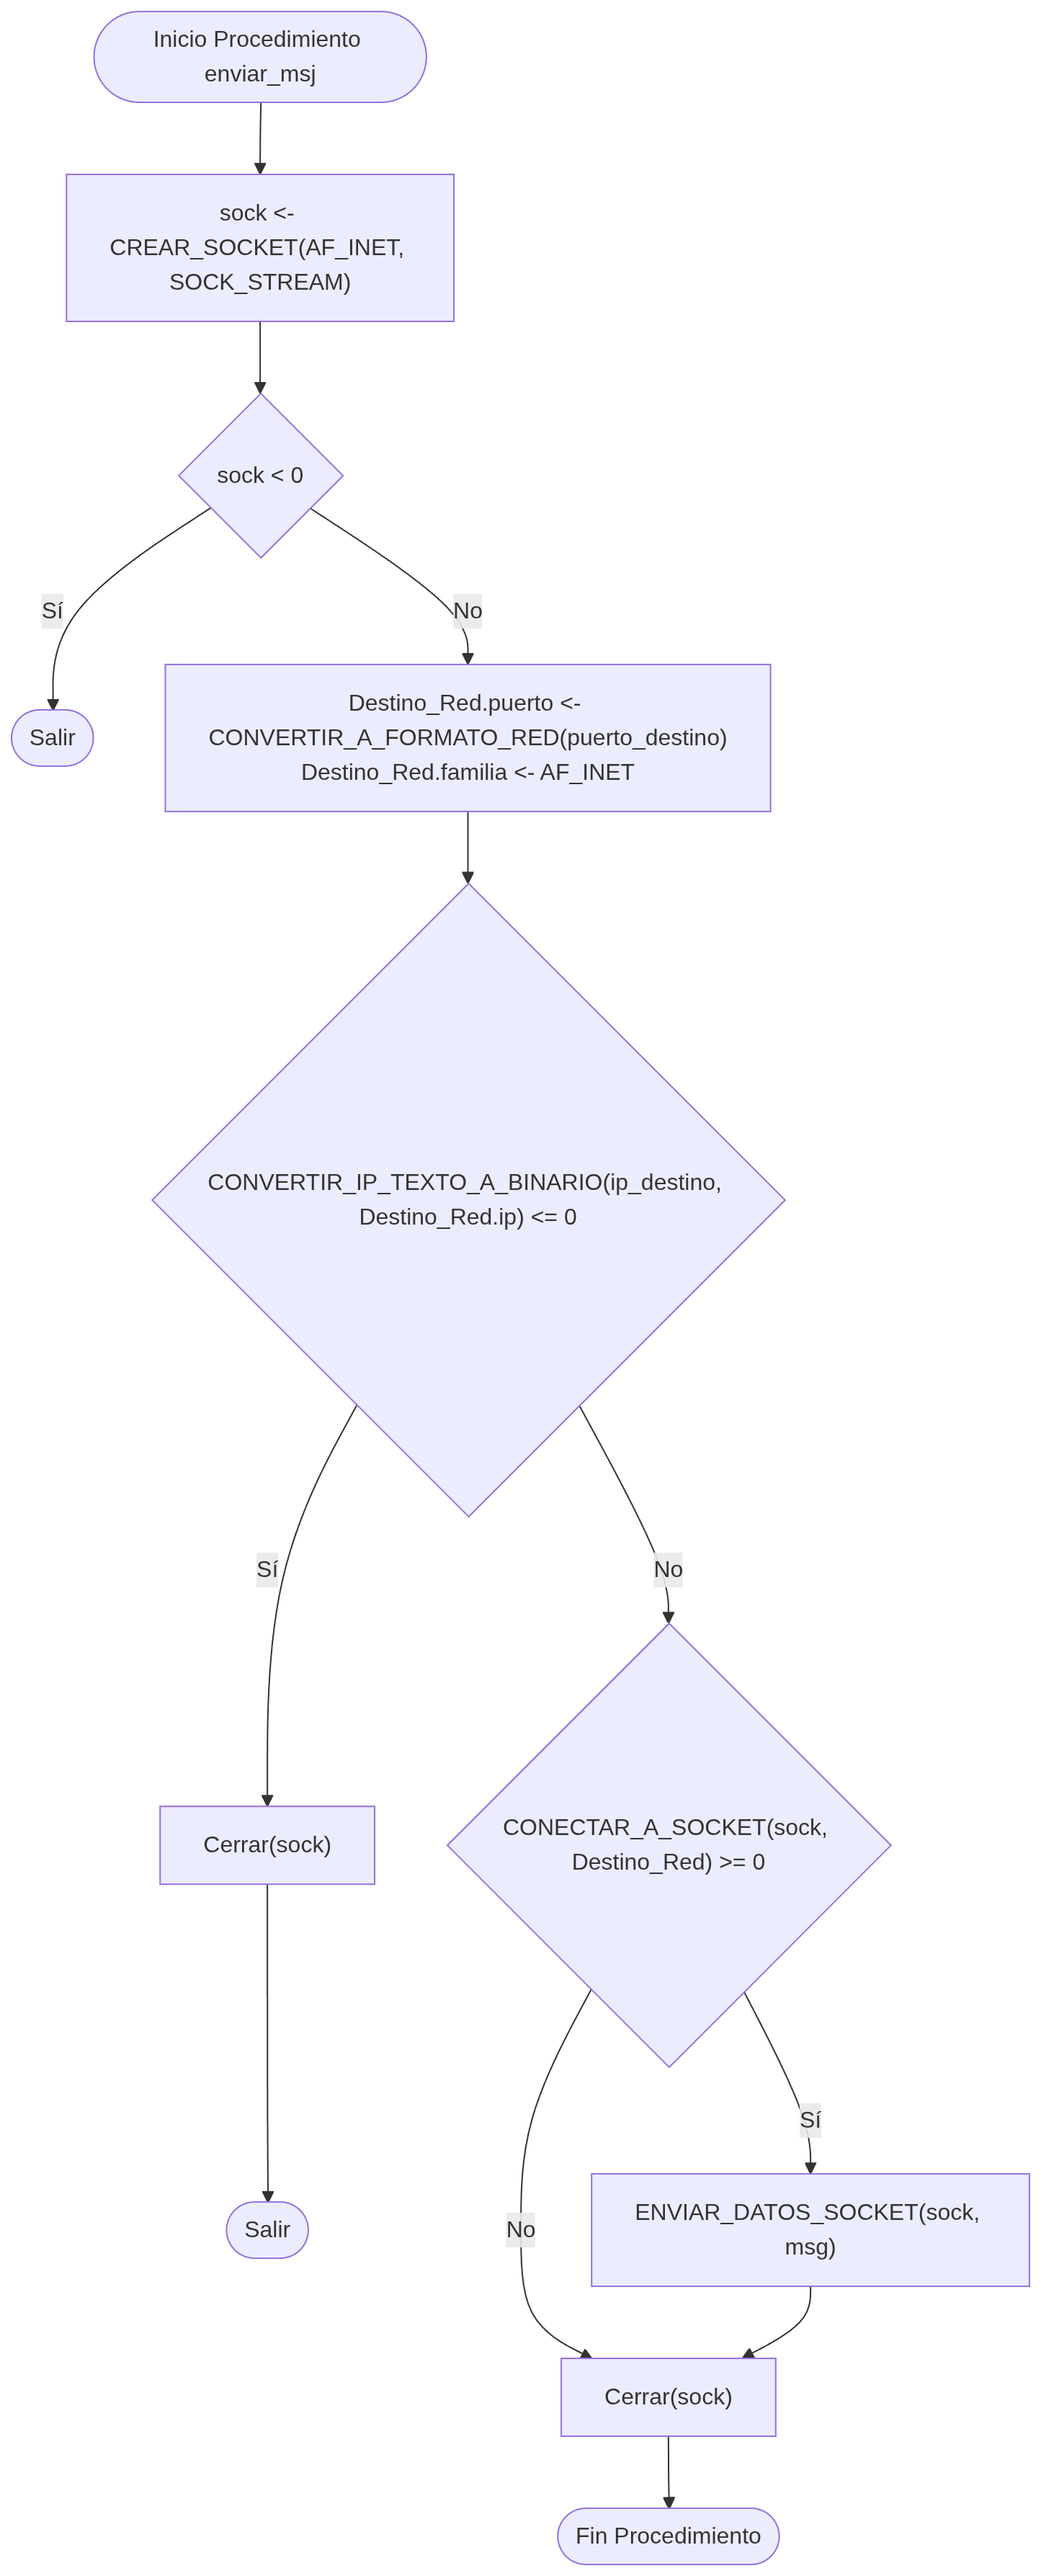
\includegraphics[width=0.4\textwidth]{Diagramas2/enviar_msj.png} 
\end{figure}

% --- FUNCION 7 Y 8 ---
\newpage
\paragraph{7. Función \texttt{get\_time\_ms()}} ~\\
\begin{figure}[H]
    \centering
    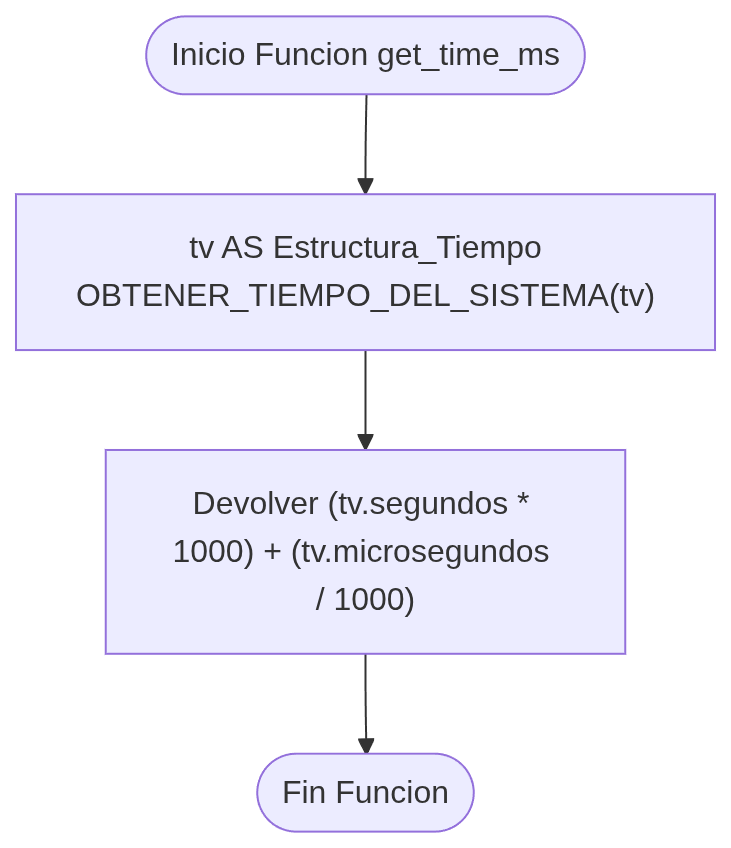
\includegraphics[width=0.25\textwidth]{Diagramas2/get_time_ms.png} 
\end{figure}

\paragraph{8. Procedimiento \texttt{formatear\_tiempo\_str()}} ~\\
\begin{figure}[H]
    \centering
    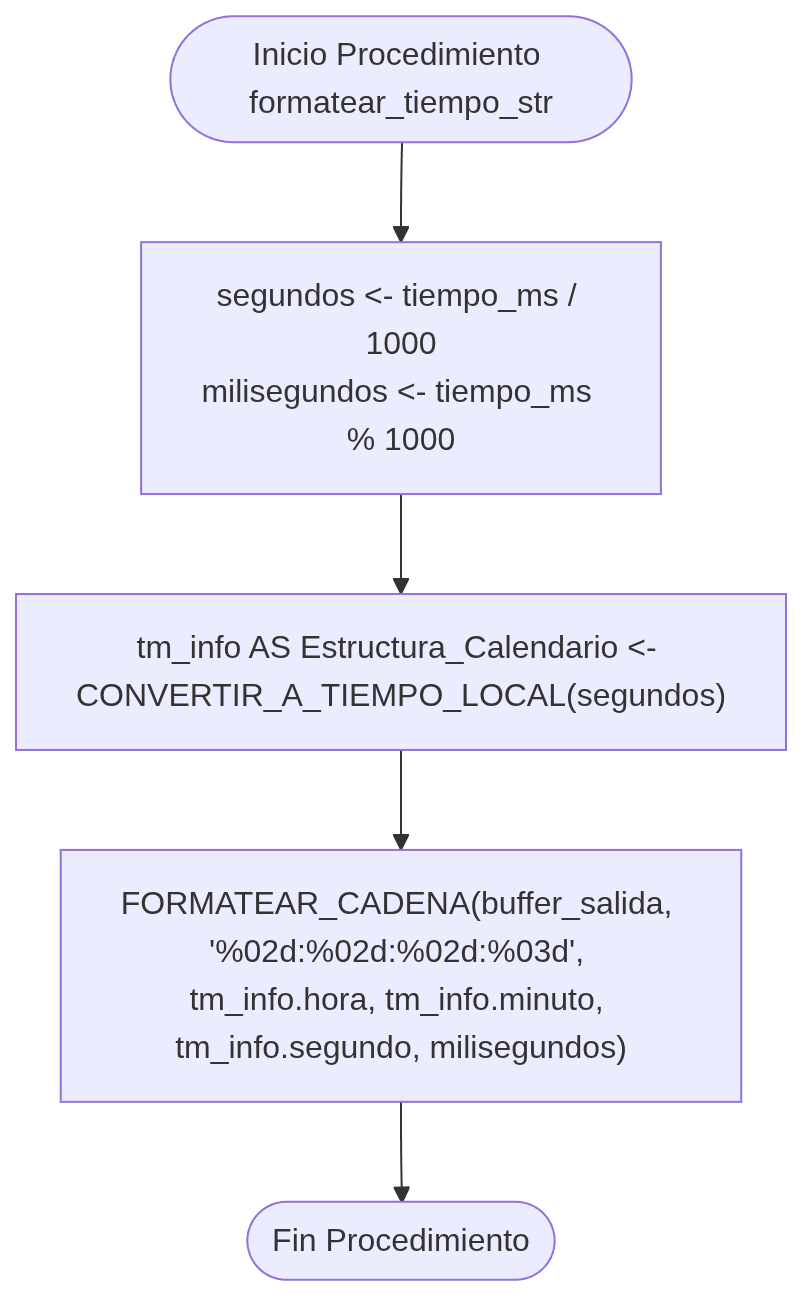
\includegraphics[width=0.25\textwidth]{Diagramas2/formatear_tiempo_str.png} 
\end{figure}